\documentclass{article} % For LaTeX2e
\usepackage{nips13submit_e, times, graphicx}

\title{Experiences implementing peer-to-peer MapReduce in the browser}

\author{Justin Huang \And Jijiang Yan}

\newcommand{\fix}{\marginpar{FIX}}
\newcommand{\new}{\marginpar{NEW}}

\nipsfinalcopy

\begin{document}

\maketitle

\begin{abstract}
MapReduce~\cite{dean2008mapreduce} is a popular tool for processing large
amounts of data. However, the average person typically doesn't have easy access
to a MapReduce implementation. This paper presents Crowd MapReduce, which allows
jobs to be created and run through a browser-based interface. The computation is
distributed across volunteers who visit a given URL, in a peer-to-peer way. We
found that our system did not deliver good performance, and discuss the
challenges involved in implementing our system.
\end{abstract}

\section{Introduction}
The typical person can run a MapReduce job in one of two ways. Either they have
access to a server cluster with some MapReduce implementation already installed
and configured, or they pay for access to a system running on a cloud provider's
servers. Both of these methods can be difficult for researchers who want to use
MapReduce, but have neither the expertise nor the resources to set it up. At the
same time, there is a trend towards crowdsourcing, where people are
increasingly willing to donate time and resources for good causes.

In response, we have designed and implemented Crowd MapReduce, which allows
people to create and run MapReduce jobs through a simple browser interface.
Instead of using dedicated servers, the computation and data are distributed in
a peer-to-peer fashion across volunteers who visit a particular URL.
Additionally, the system is implemented as a client-side application, meaning
that running the system just requires a web server to serve up static files.

\subsection{Design goals and assumptions}
The main goal of the system is to be extremely simple to use. It should enable
people to run MapReduce jobs without owning or having access to other computers
in the cloud. A secondary goal of the system is to test the limits of modern web
technologies, and see how close they are to providing a useful platform for
applications such as Crowd MapReduce.

One assumption we are making is that the job creator is reliable, and will keep
a job tracking webpage open until the job is complete. On the other hand, we
assume that volunteers are not as reliable, and may decide to disconnect at any
time.

We also assume that the user's data can be represented as text. We represent all
data as strings or arrays of strings for performance reasons.

Additionally, since the job creator is sending volunteers code to execute and
volunteers are sending data back, security may be a concern. However, we assume
that neither the job tracker nor the volunteers are malicious, and will run our
system as given.

\section{Previous work}
A similar idea was discussed in 2009 by Ilya Grigorik on his
blog~\cite{grigorik2009}. However, he only discussed the idea of such a system
without fully implementing it.

In 2010, Ryza and Wall provided an implementation of browser-based MapReduce for
a class project~\cite{mrjs}.
Langhans, Wieser, and Bry presented a similar
system~\cite{langhans2013crowdsourcing} to that of Ryza and Wall. Both systems use a centralized server, where clients request work over HTTP. This setup is
vulnerable to server failure -- if the server goes down, every job running on
the server will fail. In contrast, our system is run completely in the browser.
This means that if a job creator's browser crashes, then their job will be lost.
However, no one else's job will be affected.

\section{Implementation}
In this section, we will describe our implementation of Crowd MapReduce in
detail, by following the creation and execution of an example job.

\subsection{Job creation}
When someone wants to create a job, they go to the job creation page, shown in
figure~\ref{creationpage}. The user inputs Javascript function bodies for the
mapper and reducer, conforming to the API given in figure~\ref{api}.

\begin{figure}[h]
  \centering
    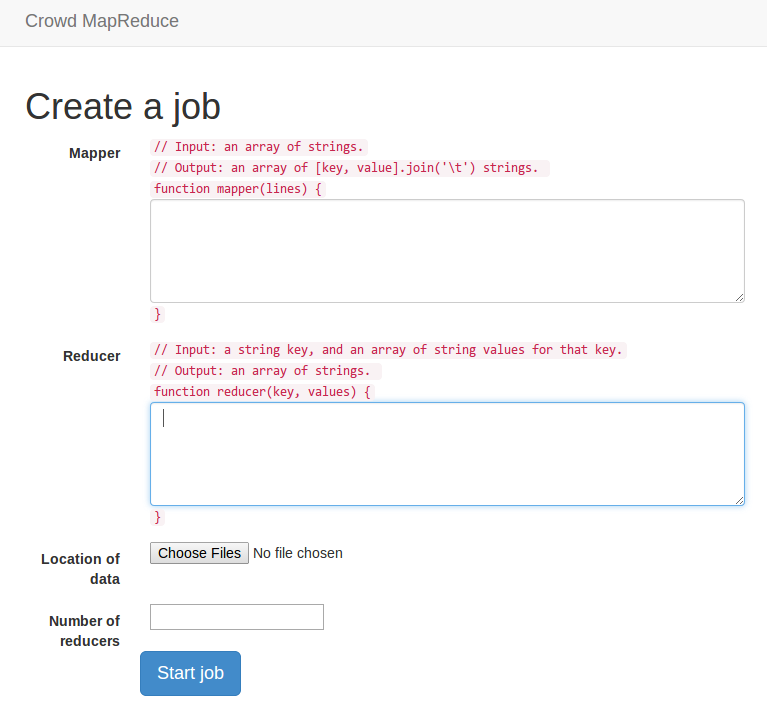
\includegraphics[width=0.75\textwidth]{create}
    \caption{A screenshot of the job creation page.}
    \label{creationpage}
\end{figure}

\begin{figure}[h]
  \begin{tabular}{| l | p{5.5cm} | p{6cm} |}
    \hline
    Function & Input & Output \\ \hline
    mapper & An array of strings & An array of key/value pairs as strings, each
    with format:
    key$<$TAB$>$value \\ \hline
    reducer & A key and an array of values, as strings & A reduced array
    of string values
    \\
    \hline
  \end{tabular}
  \caption{The API for the mapper and reducer functions.}
  \label{api}
\end{figure}

Next, the user must upload their data. Because we assume the user has no access
to cloud storage, the data is instead copied to a virtual filesystem provided by
the browser. This is only possible for browsers implementing the HTML 5
FileSystem API~\cite{html5file}. The FileSystem API allows applications to store
an arbitrary amount of data in the virtual filesystem, as long as the user
approves it.

We assume that the user's data is already broken into multiple files, such that
each file will be the input to a mapper. Hence, the number of mappers is equal
to the number of files. Our application could possibly split the user's data
automatically, given a maximum size for each map task. However, we chose not to
do this due to time constraints. This functionality is already provided by the
Unix \texttt{split} utility.

Finally, the user specifies the number of reduce partitions for the job. The
concept of reduce partitions in our system is similar to that of the Google
MapReduce implementation. More reduce partitions leads to greater parallelism,
but also leads to more output files, which the user must be prepared to combine
on their own.

\subsection{Job tracker}
Once the job has been created, the user is taken to a job tracker page, shown in
figure~\ref{maprunning}.

\begin{figure}[h]
  \centering
    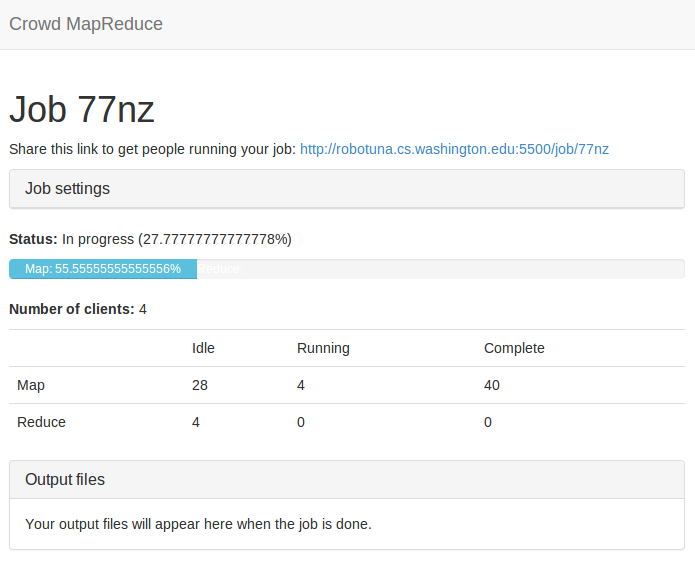
\includegraphics[width=0.75\textwidth]{maprunning}
    \caption{A screenshot of the job tracker page, showing a job in progress.}
    \label{maprunning}
\end{figure}

The job tracker provides several pieces of information:
\begin{itemize}
  \item The URL to share to volunteers.
  \item The number of volunteers who are running jobs.
  \item The progress of the job, expressed both as an overall percentage, and as
  a breakdown of the tasks that are either waiting to run, running, or complete.
  \item Download links for the output data when the job completes.
\end{itemize}

In order to establish a peer-to-peer connection between the job tracker and the
volunteers, we use another recent browser technology, WebRTC~\cite{webrtc}.
WebRTC is a browser API which allows peers to send arbitrary data to each other.
In our implementation, we used the PeerJS library~\cite{peerjs}, which
simplifies the WebRTC APIs.

The job tracker maintains two primary data structures. The first data structure
keeps track of what tasks need to be done, which tasks are running, and which
are complete. Each task specifies the location of a file on the virtual
filesystem, which contains the input data for the task. The second data
structure is a list of clients who have connected, as well as what task they
are assigned to.

When a client connects, an idle task is assigned to a client. The job tracker
loads the input data from the virtual filesystem into memory, then sends the
data and code to the client. The actions of the client are described more in the
next section.

If a client disconnects, the job tracker looks up which task they were assigned
to, and moves the task back into the idle queue. Otherwise, the client responds
with the results. For both map and reduce tasks, the results are in the form of
key/value pairs. The job tracker writes each result to one of the reduce
partitions on the filesystem based on the hash of the key.

The reduce phase does not start until all the map tasks are done. For a
sufficiently large dataset, the number of reduce partitions that were actually
written to will be the same as the number of reduce partitions the job creator
specified. When all the reduce tasks are complete, the job tracker provides
download links for the output files from the virtual filesystem.

\subsection{Job client}
The URL for a job client page contains the unique job ID necessary for the
client to connect to the job tracker. When it is a assigned a map task, it
simply evaluates the mapper code as a Javascript function, and passes in the
array of data given by the job tracker. It then returns the results of the
mapper back to the job tracker.

When the client processes a reduce task, it takes the additional step of sorting
the data and grouping the values by key. The key and the array of values are
passed to the reducer, which returns the reduced array of values. When finished,
the client sends the data back to the job tracker as a flattened list of
key/value pairs.

\section{Performance}

\section{Conclusion}

\bibliographystyle{unsrt}
\bibliography{report}

\end{document}